% !TeX root = ../defense.tex

\section{Conclusion and Outlook}
\frame{\sectionpage}

\begin{frame}{Our work in perspective}
\vskip 1cm
\begin{tikzpicture}
\uncover<+->{
	\node [terminator, fill=yellow!20] at (0,0)  (model)       {\textbf{Model selection}};
}
\uncover<+->{
	\node [terminator, fill=blue!20]   at (0,-1.5) (calculation) {\begin{minipage}{.3\linewidth}
		\centering
		Spectral energy density\\ calculation
	\end{minipage}};
	\path [connector] (model)       -- (calculation);
}
\uncover<+->{
	\node [terminator, fill=blue!20]   at (0,-3) (simulation)  {\begin{minipage}{.3\linewidth}
		\centering
		GW data simulation
	\end{minipage}};
	\path [connector] (calculation) -- (simulation);
}
\uncover<+->{
	\node [terminator, fill=blue!20]   at (0,-4.5) (analysis)    {\begin{minipage}{.3\linewidth}
		\centering
		Topological data analysis
	\end{minipage}};
	\path [connector] (simulation)  -- (analysis);
}
\uncover<+->{
	\node [decision  , fill=red!20]    at (5,-4.5) (tests)       {Tests};
	\path [connector] (analysis)    -- (tests);
}
\uncover<+->{
	\node [terminator, fill=green!20]  at (10,-2.5) (simwork)     {\begin{minipage}{.3\linewidth}
		\centering
		Checking the viability\\ of simulation
	\end{minipage}};
	\path [connector] (tests)       |- (simwork);
}
\uncover<+->{
	\node [terminator, fill=green!20]  at (10,-4.5) (noise)       {\begin{minipage}{.3\linewidth}
		\centering
		Distinguishing signal from\\ noise
	\end{minipage}};
	\path [connector] (tests)       -- (noise);
}
\uncover<+->{
	\node [terminator, fill=green!20]  at (10,-6.5) (class)       {\begin{minipage}{.3\linewidth}
		\centering
		Classifying signals\\ with different $\sigma_{PBH}$ values
	\end{minipage}};
	\path [connector] (tests)       |- (class);
}
\end{tikzpicture}
\end{frame}

\begin{frame}{General statistics}
\uncover<+->{For this work:\\~\\}
\begin{itemize}[<+->]
	\item 3600 signals for 10 different physics were simulated.\\~\\
	\item 6 different noise amplitudes were added.\\~\\
	\item Tens of embedding dimensions and time delays were tested.\\~\\
	\item Tens of topological vectorization and amplitude measures were tested.\\~\\
	\item A 10 dimensional feature vector was selected.\\~\\
	\item A 90\% classification accuracy was achieved.
\end{itemize}
\end{frame}

\begin{frame}{Innovations}
\uncover<+->{Three important innovations were made in this research:\\~\\}
\begin{itemize}[<+->]
	\item A code was written to calculate a spectral energy density using the semi-analytical formula; which is expandable to other astrophysical, cosmological and dynamical scenarios.\\~\\
	\item A number of functions and a data structure were added to the \textit{LALSuite} package which enable it to simulate a SGWB from a custom $\Omega_{SGWB}$.\\~\\
	\item A novel topological measure was introduced which can classify different SGWBs based on their physical parameters.
\end{itemize}
\end{frame}

\begin{frame}{Suggestions}
\uncover<+->{In the future we can expand on this research by doing:\\~\\}
\begin{itemize}[<+->]
	\item A Fischer forcast to evaluate the detection probability of PBH-induced SGWBs via different ovservatories.\\~\\
	\item Comparing our classification results with the results from more classical algorithms.\\~\\
	\item Considering other PBH formation scenarios and simulating their SGWBs.\\~\\
	\item Changing various astrophysical and cosmological parameters to investigate our models ability to constrain those parameters.
\end{itemize}
\end{frame}

\begin{frame}{Accessibility}
In the end, if you are interested in my research, you can sownload my thesis and see my contact information on my page at physics department's computational cosmology group website:
\vskip 2cm
\centering
\LARGE \href{http://ccg.sbu.ac.ir/people/ali-salehi/}{ccg.sbu.ac.ir/people/ali-salehi}
\end{frame}

\usebackgroundtemplate{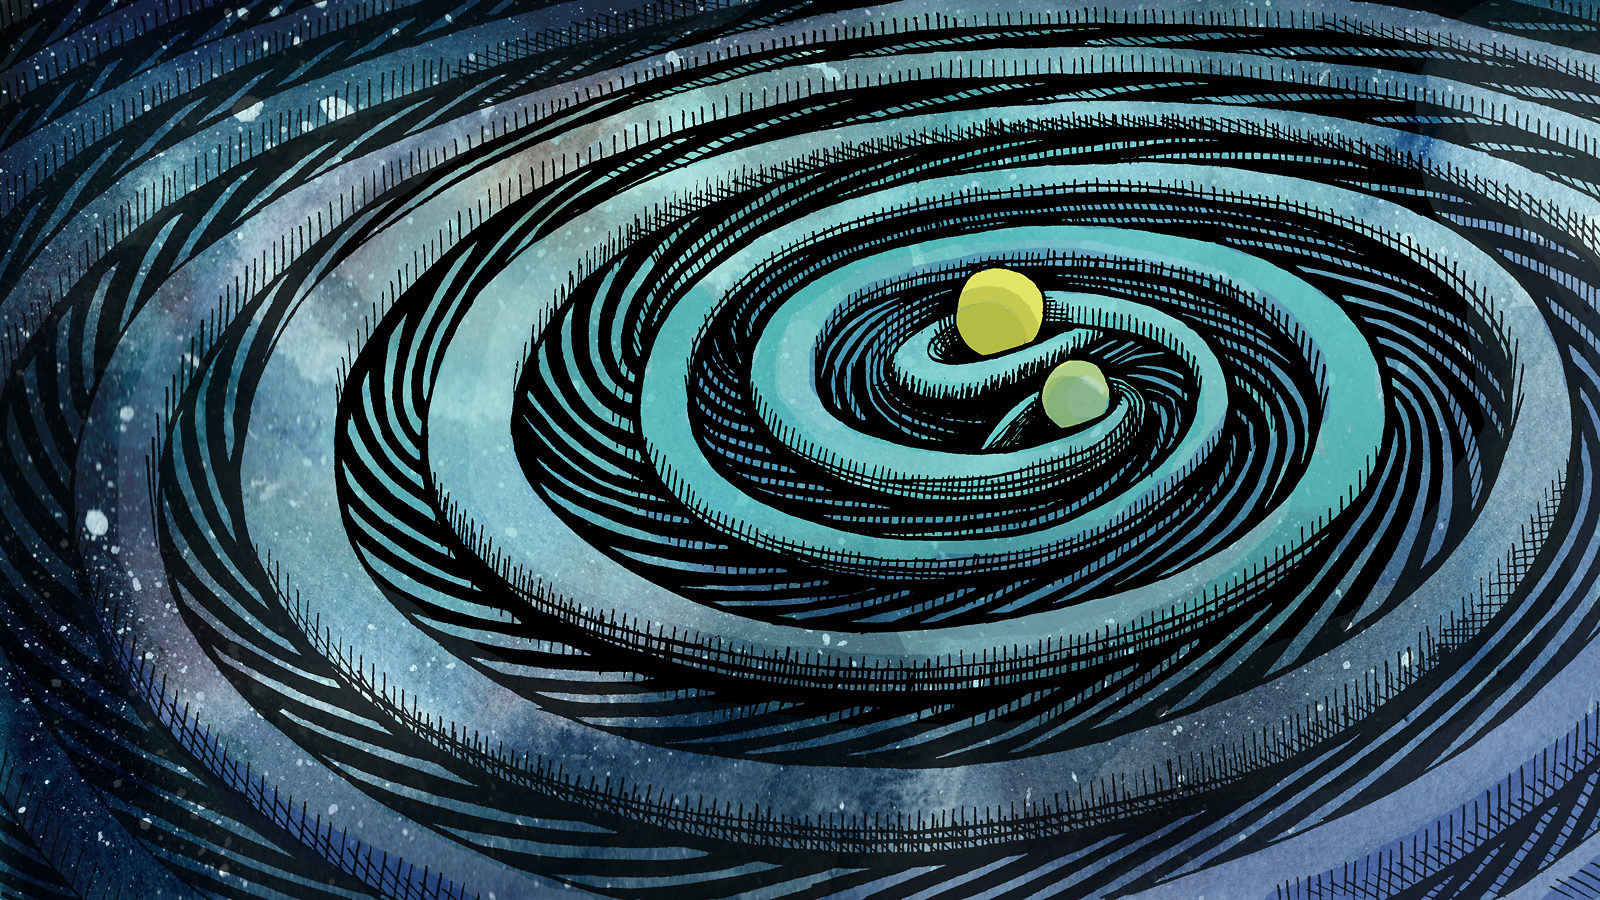
\includegraphics[height=\paperheight]{img/gw-cartoon}}
\begin{frame}[plain]
\begin{center}
\vspace*{5cm}
\contourlength{2pt} %how thick each copy is
\contournumber{20}  %number of copies
\contour{black}{\Huge \textcolor{white}{Thank you for your attention!}}\\
%\Huge \textcolor{white}{Thank you for your attention!}\\
\end{center}
\end{frame}